\documentclass[%
	%draft,
	%submission,
	%compressed,
	final, %technote,
	%internal,
	%submitted,
	%inpress,
	%reprint,
	% %titlepage,
	notitlepage,
	%anonymous,
	narroweqnarray,
	inline,
	twoside,
        %invited,
	]{ieee}

\usepackage[top=3cm, bottom=2cm, left=1.5cm, right=1.5cm,a4paper,includeheadfoot]{geometry}



\usepackage[utf8]{inputenc}			% idioma
\usepackage[spanish]{babel}
\usepackage{float}
%\usepackage{color}
%\usepackage{colortbl}
%\usepackage{amsmath}
%\usepackage{amsfonts}
%\usepackage{verbatim}

\usepackage{hyperref}				% urls

% -------- PARA FIGURAS
\usepackage{graphicx}
%\usepackage{capt-of}
% -------- FIN FIGURAS

% -------- PARA MONXTRAR EL CODIGO DE MANERA AMENA
\usepackage{courier}
\usepackage{listings}
\lstset{ %
	language=C++,                % choose the language of the code
	basicstyle=\footnotesize\ttfamily,       % the size of the fonts that are used for the code
	numbersep=5pt,                  % how far the line-numbers are from the code
%	backgroundcolor=\color{white},  % choose the background color. You must add \usepackage{color}
	showspaces=false,               % show spaces adding particular underscores
	showstringspaces=false,         % underline spaces within strings
	showtabs=false,                 % show tabs within strings adding particular underscores
	frame=single,           % adds a frame around the code
	tabsize=6,          % sets default tabsize to 2 spaces
	captionpos=b,           % sets the caption-position to bottom
	breaklines=true,        % sets automatic line breaking
	breakatwhitespace=false,    % sets if automatic breaks should only happen at whitespace
}
\usepackage{sidecap}
\usepackage{amsmath}
\usepackage{wrapfig}
\usepackage{caption}
\usepackage{subcaption}
\usepackage{tikz}
\usepackage{tikz-qtree}

\newcommand{\subsubsubsection}[1]{\paragraph{#1}\mbox{}\\}
\setcounter{secnumdepth}{4}
\setcounter{tocdepth}{4}
%\usepackage{minted}

%Formato de los links
\usepackage{hyperref}
\hypersetup{
  colorlinks   = true, %Colours links instead of ugly boxes
  urlcolor     = blue, %Colour for external hyperlinks
  linkcolor    = blue, %Colour of internal links
  citecolor   = red %Colour of citations
}
% -------- FIN CODIGO

\hypersetup{			%sacar los colores horrendos de las ref
	colorlinks=false,
	pdfborder={0 0 0},
}


\begin{document}


\title[Wiretapping]{%
	Análisis de tráfico de redes locales usando Teoría de la Información
}

\author[BALBACHAN, COSTA, GATTI]{
Alexis Balbachan \authorinfo{A. Balbachan e-mail: alexisbalbachan@gmail.com}%
\and{}Manuel Costa \authorinfo{M. Costa, e-mail: manucos94@gmail.com}%
\and{}Mathias Gatti\authorinfo{M. Gatti, e-mail: mathigatti@gmail.com}
}

%\journal{Grupo 13: Teor\'ia de las Comunicaciones, Departamento de Computaci\'on, UBA}

\firstpage{1}

\maketitle               

\begin{abstract} 
\end{abstract}

\begin{keywords}
entropía, Teoría de la informacin, ARP, LAN, unicast, broadcast, sniffing
\end{keywords}



Iniciamos este trabajo con el objetivo de aprender sobre el protocolo ARP y mas en general las redes de Internet y sus algoritmos de intercambio de paquetes.

A lo largo de este informe describiremos ciertos análisis que tendrán como objetivo el modelado de emisores de información y la detección de símbolos destacados. A partir de esta metodología creemos que podremos identificar dispositivos claves en la red como por ejemplo el gateway. Nuestra hipótesis es que este tendrá destacará en el intercambio de paquetes who-has siendo de los que mas reciba y envíe.

\section{Métodos}
\subsection*{Herramientas}
Para la captura de tráfico se utilizó el módulo de manipulación de paquetes \emph{Scapy} para python, el cual provee una interfaz sencilla para nuestros requerimientos puntuales. \emph{Scapy} permite la captura y posterior guardado de paquetes en una red, para luego ser filtrados, inspeccionados o manipulados con facilidad. Además, para incrementar la cantidad de paquetes vistos por un host, se activó el modo promiscuo o modo monitor en sus respectivas interfaces de red.

\subsection*{Modelo de las fuentes}

\subsubsection*{Fuente S1}
Dado el tráfico de capa 2 obtenido en cada captura, se modeló una fuente de memoria nula S1 = $ \{ s_{1}, s_{2}, s_{3},...,s_{n} \}$ donde cada $ s_{i} $ está formado por una tupla (broadcast $\|$ unicast), protocolo capa 3.

\subsubsection*{Fuente S2}
Para el ejercicio 2 modelamos la fuente de memoria nula S2 la cual intenta definir sus símbolos de manera que estos permitan encontrar nodos destacados a partir de herramientas de teoría de la información y los paquetes ARP de una red.

Luego de experimentar con distintas variantes posibles de los datos provistos por los paquetes ARP nos terminamos decidiendo por utilizar el destino de los paquetes who-has ya que estos a diferencia de los paquetes is-at son broadcast por lo que se propagan a través distintas subredes y switches permitiendo recibirlos en gran número lo cual genera mediciones más robustas. Por otro lado elegimos quedarnos solo con el destino ya que creemos que es una buena heurística para encontrar nodos destacados, ya que si un nodo es destacado (por ejemplo un router con salida a internet) entonces varios hosts querrán comunicarse con él, convirtiéndolo en el destino de un paquete who-has. Notar que no tendría tanto sentido utilizar la fuente ya que al menos para routers no va a ser de mucha utilidad debido a que probablemente estos ya tengan en su tabla a la mayoría de las MACs de los hosts de su red y no necesiten generar tantos paquetes ARP who-has, por esta razón este pasaría desapercibido entre los demás hosts.

\subsubsection*{Capturas}
Se hicieron 3 capturas en redes diferentes durante aproximadamente 30 minutos (Todas con al menos 10.000 tramas):
\begin{itemize}
	\item Red hogareña pequeña, con aproximadamente 10 usuarios, se utilizó una interfaz ethernet. La medición se realizó un jueves por la noche, a las 20 horas cuando la mayoría de los usuarios de la misma estaban conectados.
	\item Red mediana de oficina de una PyMe, mediciones tomadas mediante la interfaz wifi, se capturó el tráfico un miércoles a las 12 del mediodía, cuando la red estaba levemente congestionada.
	\item Red grande del laboratorio de informática de la universidad, mediciones tomadas mediante una interfaz wifi, se capturó el tráfico a las 19 horas de un miércoles en el laboratorio turing, cuando había 8 personas más utilizando las computadoras del laboratorio.
\end{itemize}


\section{Resultados y análisis}

\subsection*{Red hogareña}
\subsubsection*{Resultados fuente S1}


Los paquetes broadcast representan un poco más del $5\%$ del total, lo cual es un valor esperable en una red que ya tiene sus tablas ARP llenas y no necesita realizar tantos broadcasts.

\begin{figure}[H]
 \centering
 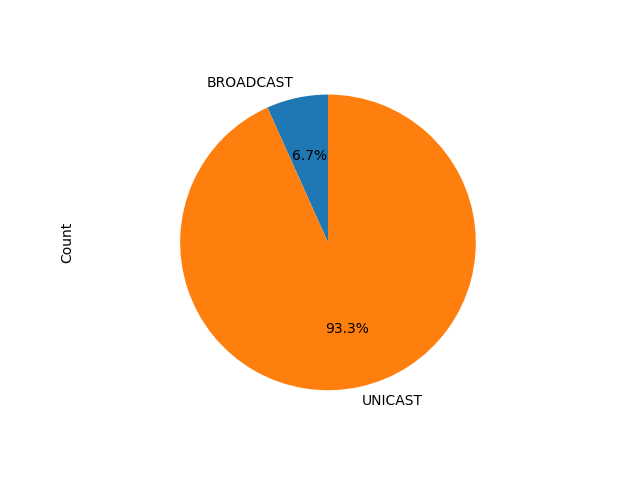
\includegraphics[width=8.5cm]{figs/broadcast_proportion_hogar_ethernet_S1_output.png}
 \caption{\normalfont Proporción de paquetes unicast/broadcast en la captura}
\end{figure}

Como se puede ver en el siguiente diagrama de torta los protocolos encontrados fueron $ARP$, este es un protocolo de resolución de direcciones, mapea direcciones $IP$ a direcciones $MAC$ (Va del nivel de red al nivel de enlaces), por otro lado esta $IPv4$ el protocolo de internet (Junto con $IPv6$) utilizado para transmitir mensajes, por ejemplo datos de usuarios, entre redes lan.

\begin{figure}[H]
 \centering
 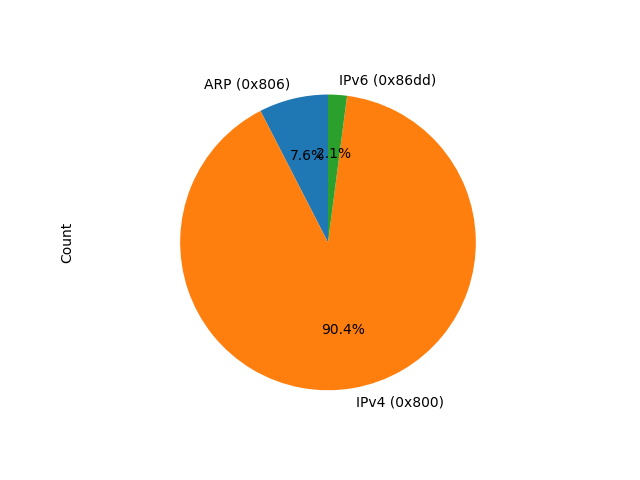
\includegraphics[width=8.5cm]{figs/protocols_proportion_hogar_ethernet_S1_output.png}
 \caption{\normalfont Proporción de protocolos en la captura}
\end{figure}

Habiendo visto el primer gráfico de torta no debería llamar la atención ver que el símbolo de menor entropía, o sea el más frecuente o de mayor probabilidad, es un unicast. Es un poco más difícil saber por qué específicamente ese protocolo tiene entropía tan baja a diferencia de los otros, posiblemente sea el protocolo mas popular visto previamente, IPv4.

Debido a este símbolo destacado también sucede que la entropía no es máxima ya que al existir este, los demás símbolos son menos probables, impidiendo la condición necesaria para la entropía máxima, que todos los símbolos sean equiprobables.

\begin{figure}[H]
 \centering
 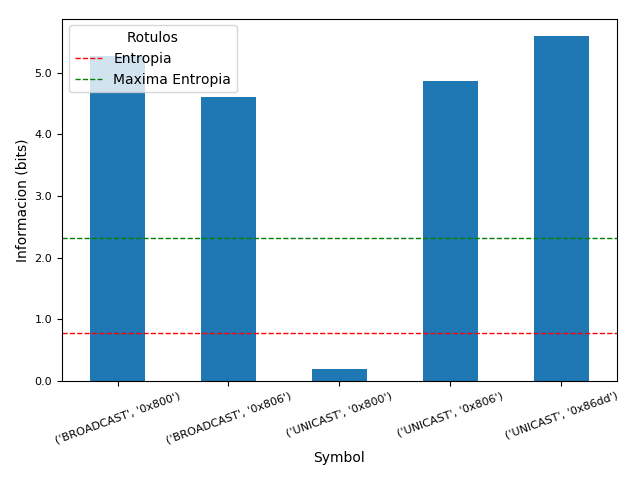
\includegraphics[width=8.5cm]{figs/information_hogar_ethernet_S1_output.png}
 \caption{\normalfont Información de los símbolos de la fuente S1, notando la entropía de la fuente, y la máxima entropía posible si la fuente fuera equiprobable.}
\end{figure}

\subsubsection*{Resultados fuente S2}

En el siguiente gráfico se pueden ver 4 hosts con baja entropía y 5 con alta entropía. Según nuestra hipótesis será de esperarse que el router sea uno de los primeros 4, idealmente el de menor entropía.

\begin{figure}[H]
 \centering
 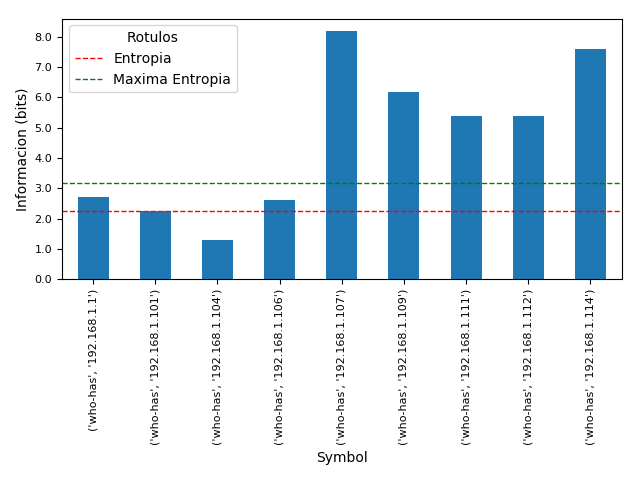
\includegraphics[width=8.5cm]{figs/information_hogar_ethernet_S2_output.png}
 \caption{\normalfont Información de los símbolos de la fuente S2, notando la entropía de la fuente, y la máxima entropía posible si la fuente fuera equiprobable.}
\end{figure}


A partir de los paquetes que se intercambian en la red armamos el grafo subyacente. En este cada vértice representa una IP local y cada arista va del origen al destino de un paquete who-has del protocolo ARP.

En este grafo los dos nodos con mayor grado son 192.168.1.1 y 192.168.1.112

\begin{figure}[H]
\centering
	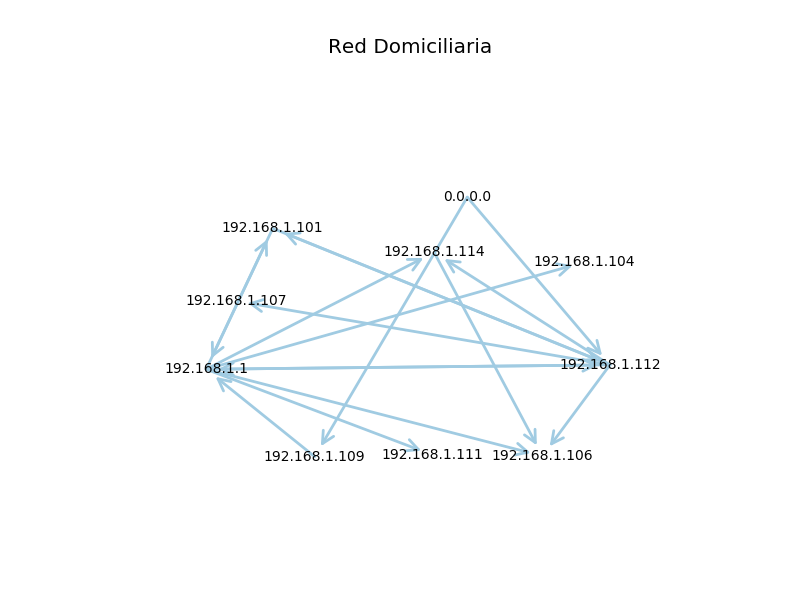
\includegraphics[width=8.5cm]{figs/grafo_red_domiciliaria.png}
	\caption{Grafo resultante de la red ethernet de una red domiciliaria durante la noche de un martes.}
	\label{fig:hogar-grafo}
\end{figure}

Cómo se puede ver si bien las dos técnicas utilizadas (Entropía y grafo subyacente) parecen apuntar a un conjunto pequeño de IPs no queda claro cuál sería el rol de cada IP o cual sería por ejemplo el router, el cual nosotros sabemos que es el 192.168.1.1, estos problemas probablemente se dan debido al tamaño de la red el cual no tiene una variedad suficientemente amplia de paquetes como para hacer robustas nuestras herramientas de predicción de símbolos destacados.

\subsection*{Red Oficina PyMe}
\subsubsection*{Resultados fuente S1}

Los paquetes broadcast representan casi el $25\%$ del total, esto es considerablemente más que en el caso anterior, una posible explicación es que la tabla de ARP de algún host se haya limpiado recientemente generando que este tenga que enviar varios who-is broadcast en la red.

\begin{figure}[H]
 \centering
 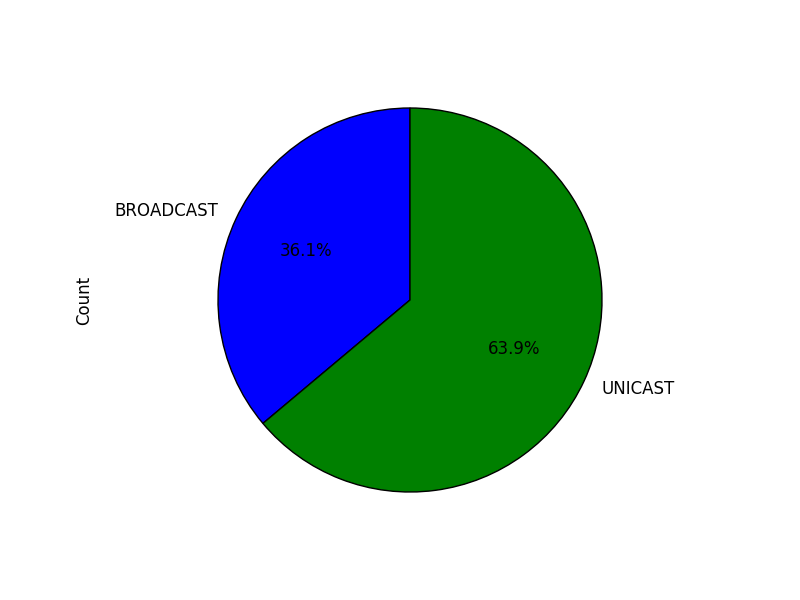
\includegraphics[width=8.5cm]{figs/broadcast_proportion_oficina_mediana_wifi_S1_output.png}
 \caption{\normalfont Proporción de paquetes unicast/broadcast en la captura}
\end{figure}

En esta red a diferencia de la anterior llegamos a ver algunos paquetes IPv6, se puede observar que este protocolo aún es mucho menos popular que el clásico IPv4. La cantidad de paquetes ARP es bastante alta apoyando la hipótesis dicha anteriormente sobre la gran cantidad de broadcasts.

\begin{figure}[H]
 \centering
 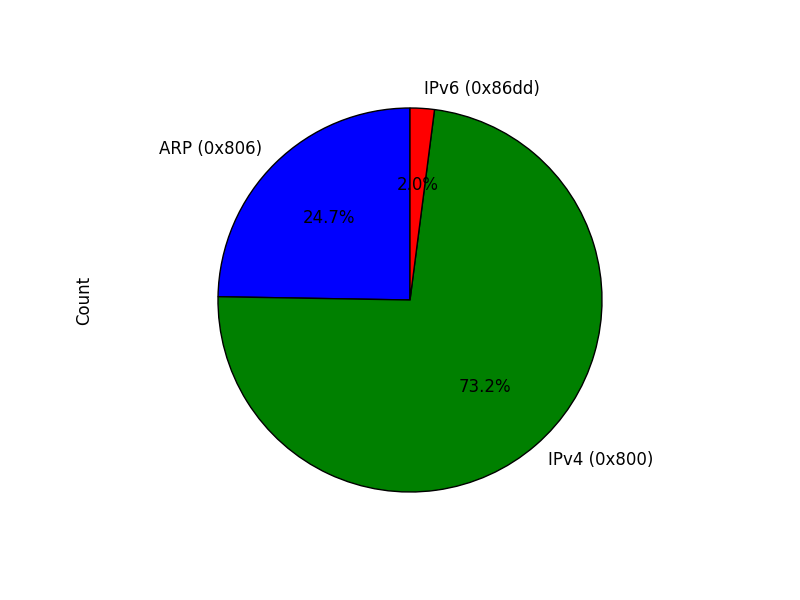
\includegraphics[width=8.5cm]{figs/protocols_proportion_oficina_mediana_wifi_S1_output.png}
 \caption{\normalfont Proporción de protocolos en la captura}
\end{figure}

El resultado es similar al visto en la red anterior dando como símbolo destacado un unicast.

\begin{figure}[H]
 \centering
 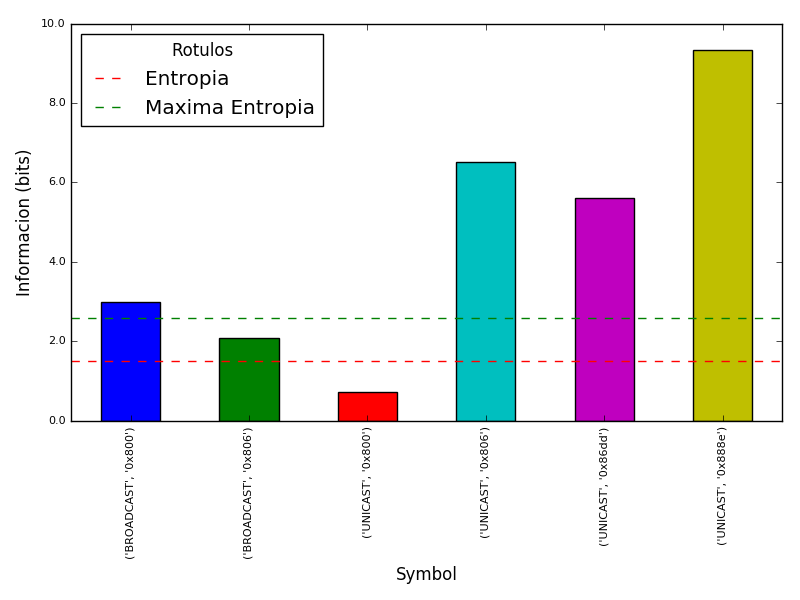
\includegraphics[width=8.5cm]{figs/information_oficina_mediana_wifi_S1_output.png}
 \caption{\normalfont Información de los símbolos de la fuente S1, notando la entropía de la fuente, y la máxima entropía posible si la fuente fuera equiprobable.}
\end{figure}

\subsubsection*{Resultados fuente S2}

En esta red hay un claro símbolo destacado con una entropía significativamente menor que la de cualquier otro.

\begin{figure}[H]
 \centering
 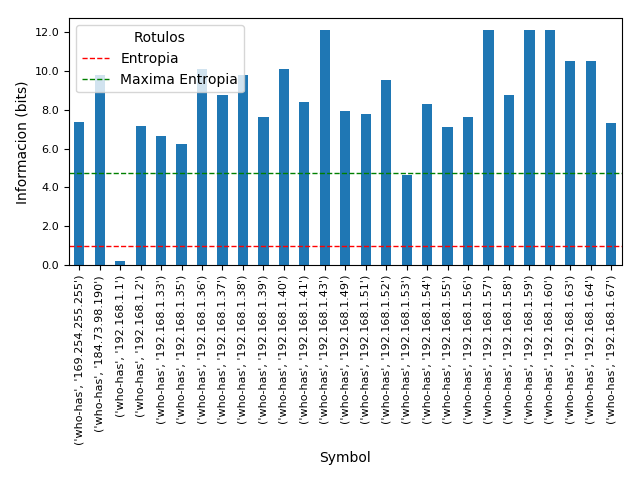
\includegraphics[width=8.5cm]{figs/information_oficina_mediana_wifi_S2_output.png}
 \caption{\normalfont Información de los símbolos de la fuente S2, notando la entropía de la fuente, y la máxima entropía posible si la fuente fuera equiprobable.}
\end{figure}

Utilizando el grafo subyacente para corroborar lo visto podemos ver que efectivamente el host 192.168.1.1 destaca (En el grafo tiene un grado mucho más alto que los demás nodos).

\begin{figure}[H]
\centering
 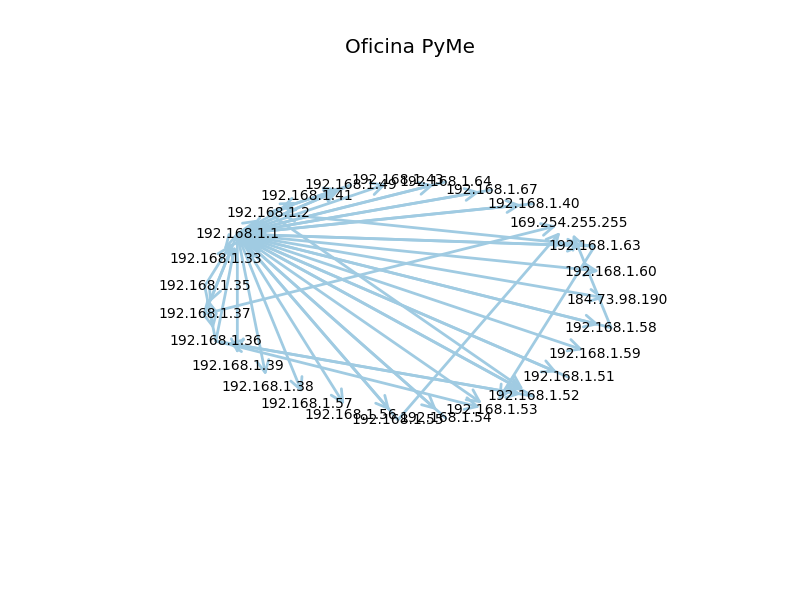
\includegraphics[width=8.5cm]{figs/grafo_pyme.png}
 \caption{Grafo resultante de la red wifi de una red pública en un starbucks durante la tarde de un día de semana.}
 \label{fig:domicilio-grafo}
\end{figure}

A diferencia del experimento con la red hogareña pudimos detectar correctamente el router de la red, esto apoya nuestra hipótesis de que el método estadístico funciona mejor con redes más grandes.

\subsection*{Red laboratorios}


\subsubsection*{Resultados fuente S1}

Al igual que con la primer red, los paquetes broadcast comprenden aproximadamente el $5\%$.

\begin{figure}[H]
 \centering
 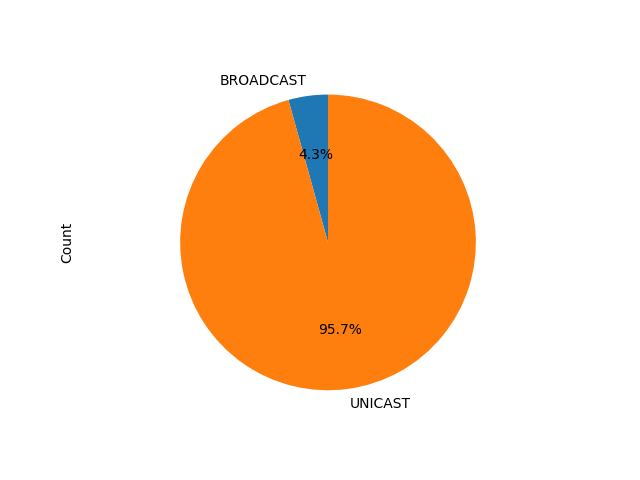
\includegraphics[width=8.5cm]{figs/broadcast_proportion_labo6_2018_04_18_S1_output.png}
 \caption{\normalfont Proporción de paquetes unicast/broadcast en la captura}
\end{figure}

Los paquetes ARP comprenden menos del $5\%$ lo cual parece indicar que la red está bastante estable. También hay algunos pocos paquetes IPv6, confirmando su escasez en comparación al protocolo IPv4.

\begin{figure}[H]
 \centering
 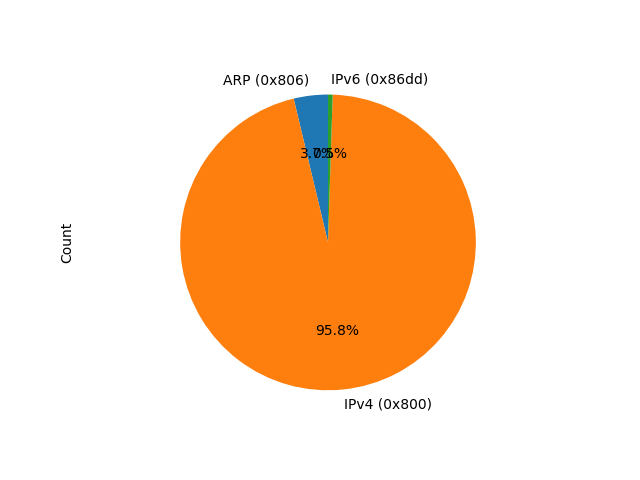
\includegraphics[width=8.5cm]{figs/protocols_proportion_labo6_2018_04_18_S1_output.png}
 \caption{\normalfont Proporción de protocolos en la captura}
\end{figure}

Al igual que en los casos anteriores el símbolo de menor entropía es un unicast de protocolo 0x800, es interesante observar como dependiendo el protocolo es tiene mayor entropía unicast o broadcast, por ejemplo con el protocolo 0x806, los broadcasts tienen menor entropía, este código posiblemente sea el de ARP por lo tanto.

\begin{figure}[H]
 \centering
 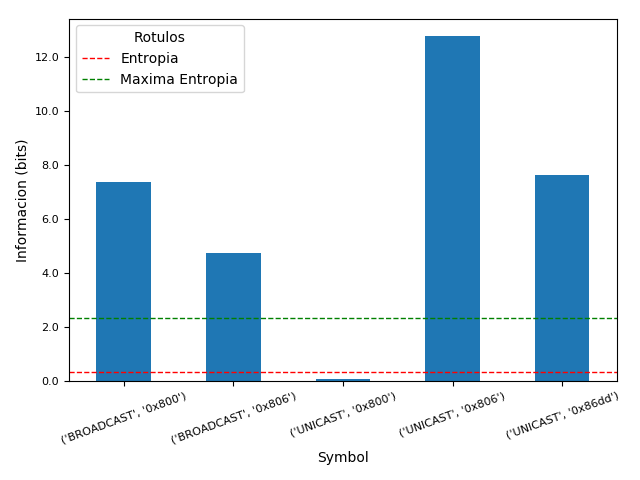
\includegraphics[width=8.5cm]{figs/information_labo6_2018_04_18_S1_output.png}
 \caption{\normalfont Información de los símbolos de la fuente S1, notando la entropía de la fuente, y la máxima entropía posible si la fuente fuera equiprobable.}
\end{figure}

\subsubsection*{Resultados fuente S2}

Destaca completamente el símbolo 10.2.203.254, este parece ser un destino muy frecuente de los paquetes who-has.

\begin{figure}[H]
 \centering
 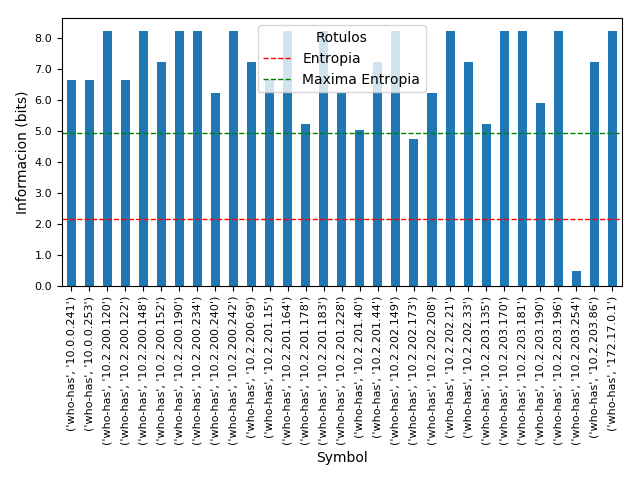
\includegraphics[width=8.5cm]{figs/information_labo6_2018_04_18_S2_output.png}
 \caption{\normalfont Información de los símbolos de la fuente S2, notando la entropía de la fuente, y la máxima entropía posible si la fuente fuera equiprobable.}
\end{figure}

En este grafo, el cual es mucho más grande que los anteriores, el nodo 10.2.203.254 es el de mayor grado corroborando lo visto en el gráfico de entropía.

\begin{figure}[H]
\centering
	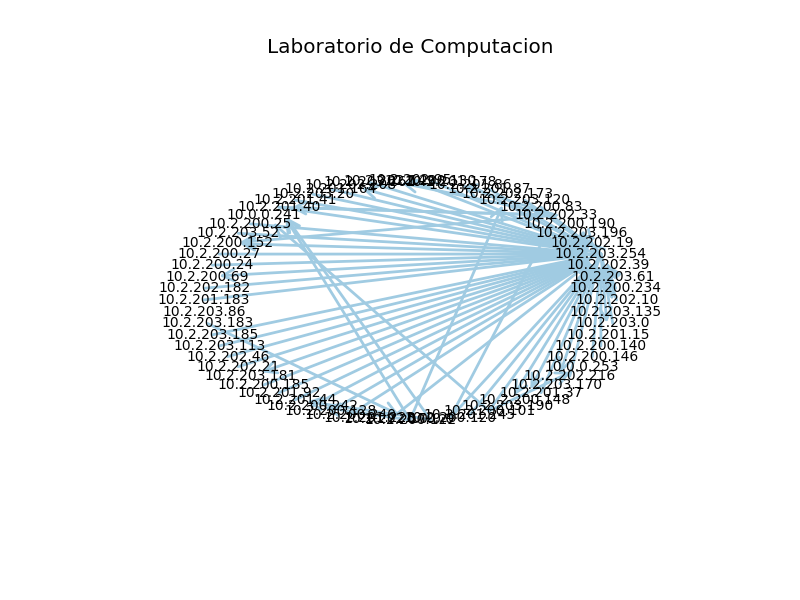
\includegraphics[width=8.5cm]{figs/grafo_dc.png}
	\caption{Grafo resultante de la red wifi del laboratorio de computación de la facultad a las 18 PM de un miércoles.}
	\label{fig:dc-grafo}
\end{figure}

De nuevo volvemos a detectar al router gracias a nuestra técnica de buscar al símbolo de menor entropía, esta parece funcionar muy bien en redes de gran tamaño.


Como resultado final pudimos identificar de distintas maneras nodos destacados, por ejemplo a partir del grafo subyacente que armamos pudimos identificar en todos los casos al gateway a partir del nodo de mayor grado. A continuación describimos brevemente cada caso analizado por separado.

\subsubsection{Red Domiciliaria}

En la red domiciliaria se pudo ver en el grafo resultante como destacaban dos nodos. Uno de ellos, el de mayor grado, era el gateway, el otro creemos que fue la computadora que tomó las mediciones ya que estaba accediendo a multiples sitios de internet lo cual provoco un gran intercambio de paquetes.

\subsubsection{Starbucks}

Quizas por una mala configuración de la red o por la poca clientela que había en este local en el horario en que se tomaron las mediciones (7:10 AM) es que este grafo resultó ser tan pobre, de todas maneras se pueden observar perfectamente los dos nodos que uno esperaría ver como minimo. El gateway y la computadora que tomo las mediciones.

\subsubsection{Laboratorio de Computación}

Este es el grafo mas grande y en el cual se vuelve aún mas claro el patrón que veniamos viendo, el nodo 10.2.203.254 resalta completamente de los demás y concuerda perfectamente con nuestra hipótesis de que el gateway es el que mas paquetes intercambia en este protocolo, lo cual lo vuelve un nodo destacado.

%----------------------------------------------------------------------

%\begin{thebibliography}{1}

%\bibitem{enunciado}
%C\'atedra de Teor\'ia de las Comunicaciones\\
%\newblock {\em Primer trabajo pr\'actico}\\
%\newblock Primer cuatrimestre $2013$

%\bibitem{arp}
%RFC 826 - Ethernet Address Resolution Protocol\\
%\url{http://tools.ietf.org/html/rfc826}\\
%\newblock C. Plummer $1982$

%\bibitem{conflicto}
%RFC 5227 - IPv4 Address Conflict Detection\\
%\url{http://tools.ietf.org/html/rfc3927}\\
%\newblock S. Cheshire $2008$

%\bibitem{link}
%RFC 3927 - Configuration of IPv4 Link-Local Addresses\\
%\url{http://tools.ietf.org/html/rfc3927}\\
%\newblock Cheshire, et al. $2005$

%\bibitem{patente}
%Method and apparatus for detecting a router that improperly responds to ARP requests\\
%\newblock US 7729292 B2\\
%\url{http://www.google.com/patents/US7729292}\\
%\newblock Stuart D. Cheshire y Joshua V. Graessley

%\bibitem{scapy}
%\texttt{Scapy}\\
%\url{http://www.secdev.org/projects/scapy}

%\bibitem{dhcp}
%RFC 1531 - Dynamic Host Configuration Protocol\\
%\url{https://tools.ietf.org/html/rfc1531}

%\bibitem{tcp}
%\url{http://www.tcpdump.org}

%\end{thebibliography}


\end{document}

